\chapter{Bandera~: génération de modèles à partir de code source Java}

\paragraph{}
Bandera~\cite{bandera1} est un logiciel permettant d'analyser un
projet Java et d'en extraire un modèle utilisable par un vérificateur
de modèle. Il a été développé suite à la collaboration de chercheurs de
l'Université d'Hawaï et de l'Université d'État du Kansas.

\paragraph{}
Ce logiciel n'est plus maintenu depuis 2005, néanmoins il peut être
intéressant de voir les décisions prises par ses développeurs pour
réaliser ce programme, en effet notre projet possède certaines
similarités~: nous cherchons aussi à analyser du code source Java afin
d'en extraire un automate.

\paragraph{}
La vérification de modèle est un problème parallèle au nôtre~: il
s'agit de vérifier si le modèle représentant un système (informatique,
mais aussi matériel) admet certaines propriétés. Par exemple,
Wikipédia cite \textit{<<~on souhaite vérifier qu'un programme ne se
  bloque pas, qu'une variable n'est jamais nulle,
  etc.~>>}\footnote{\url{https://fr.wikipedia.org/wiki/Vérification_de_modèles}}

\paragraph{}
Nous allons donc étudier son fonctionnement afin de comprendre comment
il fonctionne et possiblement s'en inspirer pour notre propre projet.

\section{Postulat de base}

\paragraph{}
Les développeurs de Bandera partent d'un constat~: des programmes de
vérification de modèle existent déjà, ils permettent de comparer un
modèle représentant un programme à un modèle de
référence. Malheureusement, créer ce modèle à la main est un travail
long, fastidieux et sujet à des erreurs humaines. De plus, chaque
vérificateur attend le modèle dans son propre langage ou format de
fichier, ce qui signifie que pour vérifier un programme avec plusieurs
vérificateurs, il faut effectuer ce travail plusieurs fois.

\paragraph{}
Leur but était donc d'écrire un programme permettant d'éliminer
l'humain de l'équation en analysant le code source et en générant des
fichiers lisibles par les vérificateurs.

\section{Fonctionnement de Bandera}
\subsection{Fonctionnement général}

\paragraph{}
Bandera est composé de quatre composants principaux qui seront pour la
plupart détaillés dans ce chapitre~:

\begin{description}
\item[Découpage du code (Section~\ref{sec:bandera_slicing})] Le découpage de code permet de supprimer les
  données et les points de contrôle qui ne sont pas nécessaires à la
  vérification d'une certaine propriété.
\item[Abstraction des variables (Section~\ref{sec:bandera_abstraction})] Bandera peut rendre certaines
  variables abstraites et les remplacer par des opérations possibles
  sur cette variable.
\item[Transformation du code source (Section~\ref{sec:bandera_source})] Afin de générer un fichier
  compatible avec les vérificateurs de modèle, Bandera passe par une
  représentation propre à ses outils.
\item[Interface graphique] Bandera est utilisable grâce à une
  interface graphique, mais celle-ci ne sera pas détaillée car elle
  n'est pas nécessaire à la compréhension de son fonctionnement.
\end{description}

\paragraph{}
La Figure~\ref{fig:desc_bandera_site}, issue du site officiel de
Bandera, détaille l'utilisation de Bandera et son fonctionnement.

\begin{figure}[H]
  \centering
  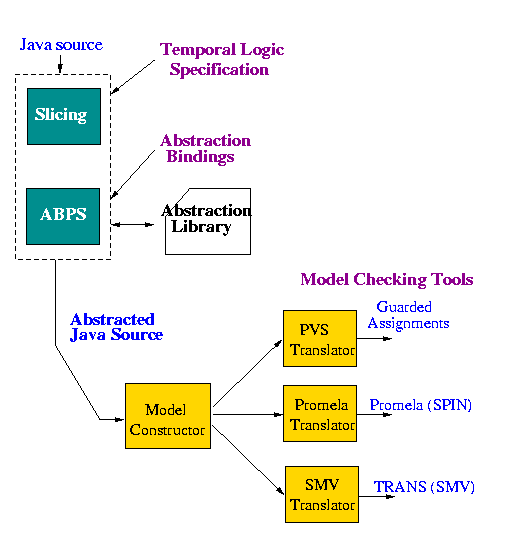
\includegraphics[scale=0.5]{images/bandera_desc.png}
  \caption{\label{fig:desc_bandera_site} Schéma de fonctionnement de Bandera}
   Source: \url{http://bandera.projects.cs.ksu.edu}
\end{figure}


\subsection{Découpage (\textit{slicing}) du programme}
\label{sec:bandera_slicing}

\paragraph{}
Dans le but de ne garder que les instructions intéressantes à la
vérification d'une certaine propriété, Bandera effectue un découpage
des instructions. Pour un programme $P$, des opérations $s_i$ sont
extraites et regroupées dans $C$.

$$C = \{s_1, s_2, \ldots, s_k\}$$

\paragraph{}
Le découpage du programme va réduire $P$ afin de ne laisser que les
instructions nécessaires au bon fonctionnement des opérations
contenues dans $C$, et supprimer les autres.

\paragraph{}
Bandera se sert de cette méthode pour vérifier qu'un programme $P$
adhère à une spécification $\Phi$. Le logiciel supprime les
instructions de $P$ qui n'influent pas la satisfaction de $\Phi$. Si
$\Phi$ est juste pour la version réduite de $P$, alors $\Phi$ est
juste pour la version complète de $P$.

\paragraph{}
Découper un programme permet aussi de simplifier le travail du
vérificateur de modèle en réduisant le nombre d'instructions à
vérifier. Bandera peut ainsi générer un modèle différent en fonction
de la propriété à tester.

\subsection{Abstraction des variables}
\label{sec:bandera_abstraction}

\paragraph{}
Bandera est capable de considérer des variables et méthodes comme
\textit{abstraites}, ce qui signifie que leur valeur concrète n'est
pas spécifiée. Cette abstraction permet de réduire la taille du modèle
et de simplifier le travail du vérifieur.

\paragraph{}
Cette abstraction est effectuée par le \gls{babs}, un composant
spécialisé de Bandera. Lorsqu'une variable est définie abstraite, elle
n'est plus représentée par sa valeur mais par certaines
propriétées. Ces propriétés dépendent de la spécification, par exemple
si une variable de type \verb|ArrayList| est abstraite et qu'on ne
fait que vérifier si une valeur est contenue dedans, elle peut être
remplacée par l'abstraction
$\{ ElementPresentDansListe, ElementAbsentDansListe \}$. Dans ce cas
précis, le \gls{babs} remplacera toutes les actions effectuées sur
l'\verb|ArrayList| par des versions abstraites manipulant des symboles
représentant des deux valeurs possibles, $ElementPresentDansListe$ et
$ElementAbsentDansListe$.

\paragraph{}
Si une opération impossible à représenter par ces deux valeurs est
demandée, par exemple \verb|ArrayList.size()|, alors l'abstraction
renvoie une valeur spéciale notée $\top$. Cette valeur est ensuite
propagée dans le reste du programme, et Bandera s'occupe d'informer le
constructeur de modèle qu'il sera nécessaire d'implémenter un test
non-déterministe quand cette variable sera utilisée.

\subsection{Transformation du code source}
\label{sec:bandera_source}

\paragraph{}
Afin de transformer du code Java en un langage utilisable par des
vérificateurs, Bandera passe par un certain nombre de langages
intermédiaires. Il commence par traduire le programme en Jimple, un
langage utilisé par le framework Soot et établit des correspondances
entre le code Java et le code Soot. Ceci permet au logiciel de
retrouver le n\oe{}ud Java correspondant à n'importe quel n\oe{}ud
dans Jimple.

\paragraph{}
L'arrière-plan (\textit{backend}) de Bandera s'occupe de traduire le
code Jimple en \gls{bir}, un langage bas niveau qui abstrait les
concepts communs à de nombreux logiciels de vérification de modèle. Le
but ce ce langage intermédiaire est de pouvoir ensuite exporter le
\gls{bir} dans différents langages spécialisés pouvant être utilisés
par les vérificateurs de modèles. La traduction est faite par
\gls{birc}. Cette étape intermédiaire est très importante dans la
«~philosophie~» Bandera~: en effet, pour pouvoir exporter le résultat
de l'analyse vers un nouveau vérificateur de modèle, il est seulement
nécessaire d'écrire un greffon pour Bandera convertissant le langage
\gls{bir} en un fichier utilisable par ce nouveau vérificateur.

\paragraph{}
Ce fonctionnement est schématisé dans la figure~\ref{fig:bir_jimple}.

\begin{figure}[H]
  \centering
  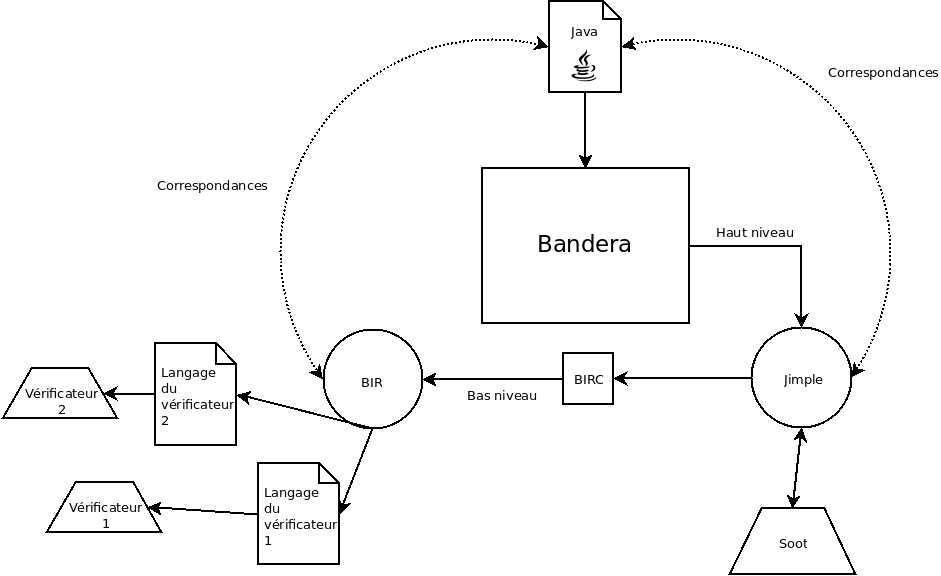
\includegraphics[scale=0.5]{images/bandera_bir_jimple.png}
  \caption{\label{fig:bir_jimple} Transformation du code source en
    langages intermédiaires}
\end{figure}

\section{Le framework Soot}

\paragraph{}
Comme vu précédemment, Bandera utilise
Soot\footnote{https://sable.github.io/soot/}\cite{Soot} afin de
convertir le code source Java du projet en Jimple, un langage
intermédiaire.

\paragraph{}
Soot est un framework permettant l'analyse de code source ou de
bytecode Java. \` A l'origine, Soot était un framework dédié à
l'optimisation de code. Au fil des versions, il s'est généralisé et
peut maintenant être utilisé pour instrumenter du code Java et le
visualiser en plus de l'optimiser.

\paragraph{}
Une comparaison entre du bytecode Java et du code Jimple est montrée
dans la Figure~\ref{fig:jimple_ex}.

\begin{figure}[ht]
  \centering
  \begin{framed}
    \center{Bytecode Java}
\begin{verbatim}
iload 1  // mets la variable x1 sur la pile
iload 2  // mets la variable x2 sur la pile
iadd     // dépile les deux valeurs et empile leur somme
istore 1 // dépile et mets la valeur dans x1
\end{verbatim}
  \end{framed}

  \begin{framed}
    \center{Source Jimple}
\begin{verbatim}
stack1 = x1 // iload 1
stack2 = x2 // iload 2
stack1 = stack1 + stack2 // iadd
x1 = stack1 // istore 1
\end{verbatim}
  \end{framed}
  \caption{\label{fig:jimple_ex} Comparaison entre du bytecode Java et Jimple}
  Source~: \url{https://en.wikipedia.org/wiki/Soot_(software)}
\end{figure}


\section{Interêt et limites}

\paragraph{}
Bandera est un outil très puissant et complexe qui gère même l'analyse
de threads Java. Les développeurs de Bandera ont choisi de ne pas
utiliser JDart (présenté dans la section suivante) pour effectuer
l'analyse afin de pouvoir modifier plus simplement le moteur d'analyse
lorsque de nouvelles avancées seront disponibles. JDart est pourtant
un outil très puissant et toujours maintenu permettant d'analyser des
applications Java.

\paragraph{}
Un des grands points forts de Bandera est de pouvoir exporter le
résultat de son analyse vers de nombreux vérificateurs de
modèle. C'est d'ailleurs son utilisation première, cette application
ayant été développée pour être compatible avec le plus de
vérificateurs possibles.

\paragraph{}
Afin de nous simplifier la tâche, nous avons décidé d'utiliser JDart,
qui sera présenté dans la prochaine section. Cet outil génère des
fichiers pour Java PathFinder en utilisant la méthode de l'exécution
concolique.

L'API JavaCard ne gérant pas les threads dans sa version
classique (ceux-ci existent dans la version Connected
Edition\footnote{\url{https://fr.wikipedia.org/wiki/Java_Card\#Version_Java_Card_3_.C2.AB.C2.A0Connect.C3.A9e.C2.A0.C2.BB}}),
toute la complexité de Bandera autour de l'analyse des fils
d'exécution ne nous concerne pas non plus.

\paragraph{}
Il apparaît que Bandera est un projet très intéressant pour la
vérification formelle de code. Cependant, la plupart des
fonctionnalités qui nous intéressent --- l'analyse du code, des
changements des variables, etc. --- sont aussi réalisables en
utilisant l'outil JDart, qui sera présenté dans la prochaine
section. Celui-ci est encore maintenu et est plus orienté vers les
développeurs, il sera donc plus simple à intégrer à notre projet.

\paragraph{}
Une autre partie intéressante de Bandera est son utilisation du
framework Soot. Ce dernier est un outil permettant l'analyse et la
modification de code source Java ainsi que de bytecode. Celui-ci
pourrait nous être utile conjointement avec JDart pour extraire les
variables participant aux changements d'état d'un applet JavaCard et
les annoter. En effet, les variables à analyser par JDart doivent être
annotées par un \verb|@Symbolic|, ce framework nous permettrais
d'effectuer ceci automatiquement.
